\documentclass[runningheads]{llncs}
\synctex=1

%=================================================================
% 
\newcount\DraftStatus  % 0 suppresses notes to selves in text
\DraftStatus=0   % TODO: set to 0 for final version
%=================================================================

%=================================================================
\usepackage{comment}
%=================================================================
%
\excludecomment{JournalOnly}  
\includecomment{ConferenceOnly}  
\excludecomment{TulipStyle}
%
%=================================================================
%=================================================================
% gitlatexdiff
%
%  https://gitlab.com/git-latexdiff/git-latexdiff
%=================================================================
%  git latexdiff HEAD  HEAD~5 --main templatex.tex
%  git latexdiff HEAD~1  --main templatex.tex
%  View pdf to see difference
%
%=================================================================
%
% Todo Notes for marginal comments
% 
%\newcount\DraftStatus  % 0 suppresses notes to selves in text
%\DraftStatus=1   % TODO: set to 0 for final version
\ifnum\DraftStatus=1
	\usepackage[draft,colorinlistoftodos,color=orange!30]{todonotes}
\else
	\usepackage[disable,colorinlistoftodos,color=blue!30]{todonotes}
\fi 
%\usepackage[disable]{todonotes} % notes not showed
%\usepackage[draft]{todonotes}   % notes showed
%
\makeatletter
 \providecommand\@dotsep{5}
 \def\listtodoname{List of Todos}
 \def\listoftodos{\@starttoc{tdo}\listtodoname}
 \makeatother
%
%=================================================================
%
\usepackage{color}
\newcommand{\draftnote}[3]{ 
	\todo[author=#2,color=#1!30,size=\footnotesize]{\textsf{#3}}	}
% TODO: add yourself here:
%
\newcommand{\gangli}[1]{\draftnote{blue}{GLi:}{#1}}
\newcommand{\qwu}[1]{\draftnote{red}{QWu:}{#1}}
\newcommand{\gliMarker}
	{\todo[author=GLi,size=\tiny,inline,color=blue!40]
	{Gang Li has worked up to here.}}
\newcommand{\qwuMarker}
	{\todo[author=QWu,size=\tiny,inline,color=red!40]
	{Qiong Wu has worked up to here.}}
%=================================================================

%=================================================================
%
% general packages
%  https://en.wikibooks.org/wiki/Category:Book:LaTeX
%  https://en.wikibooks.org/wiki/LaTeX/Package_Reference
%
%=================================================================
\usepackage{graphicx}
\graphicspath{{./figures/}{./graphics/}{./graphics/logos/}}

\usepackage{algorithm}
\usepackage{algorithmic}
\usepackage{breqn}
\usepackage{subcaption}
\usepackage{multirow}
\usepackage{psfrag}
\usepackage{url}
\usepackage[colorlinks,citecolor=blue]{hyperref}
%\usepackage{hyperref}
%\usepackage[colorlinks]{hyperref}
%\usepackage{cite}
\usepackage{cleveref}
\usepackage{booktabs}
\usepackage{rotating}
\usepackage{colortbl}
\usepackage{paralist}
%\usepackage{geometry}
\usepackage{epstopdf}
\usepackage{nag}
\usepackage{microtype}
\usepackage{siunitx}
\usepackage{nicefrac}
%\usepackage{breakurl}
\usepackage{fontawesome}
\usepackage{xcolor}
\usepackage{multicol}
\usepackage{wrapfig}
\usepackage{todonotes}
\usepackage{tablefootnote}
\usepackage{threeparttable}
% \usepackage{bibunits} 
% for random text
\usepackage{cite}
\usepackage{lipsum}
\usepackage[english]{babel}
\usepackage[pangram]{blindtext}
% for tikz figures
\usepackage{tikz}
\usetikzlibrary{fit,positioning,arrows.meta,shapes,arrows}
%\tikzset{neuron/.style={circle,thick,fill=black!25,minimum size=17pt,inner sep=0pt},
%	input neuron/.style={neuron, draw,thick, fill=gray!30},
%	hidden neuron/.style={neuron,fill=white,draw},
%	hoz/.style={rotate=-90}}
%
%=================================================================



\begin{TulipStyle}
\usepackage[numbers]{natbib}
%=================================================================
%
% Version control information
%
%=================================================================
\usepackage{gitinfo2}
%=================================================================
\usepackage{fancyhdr}
\pagestyle{fancy}
\fancyhead{} % clear all header fields
\fancyhead[RO,LE]{\textsl{\rightmark}}
\fancyhead[LO,RE]{\ensuremath{\Rightarrow}
		\textbf{\textbf{[CONFIDENTIAL]}}\ensuremath{\Leftarrow}}
\fancyhead[CO,CE]{}
%=================================================================
\fancyfoot{} % clear all footer fields
\fancyfoot[CE,CO]{\textbf{\thepage}} 
\fancyfoot[LO,LE]{
\includegraphics[height=.9\headheight]
{./graphics/logos/tulip-logo.eps}
		\gitVtagn-\gitBranch\ (\gitCommitterDate)}
\fancyfoot[RO,RE]{Committed by: \textsl{\gitCommitterName}}

\setlength{\headheight}{12pt}
\renewcommand{\headrulewidth}{0.4pt}
\renewcommand{\footrulewidth}{0.4pt}
%=================================================================


%=================================================================
% for math notations
% ----------------------------------------------------------------
\usepackage{mathtools}
\usepackage{amsthm}
%
% THEOREMS -------------------------------------------------------
%
\newtheorem{thm}{Theorem}[section]
\newtheorem{cor}[thm]{Corollary}
\newtheorem{lem}[thm]{Lemma}
\newtheorem{prop}[thm]{Proposition}
\theoremstyle{definition}
\newtheorem{defn}[thm]{Definition}
\theoremstyle{remark}
\newtheorem{rem}[thm]{Remark}
\numberwithin{equation}{section}
% MATH -----------------------------------------------------------
\newcommand{\norm}[1]{\left\Vert#1\right\Vert}
\newcommand{\abs}[1]{\left\vert#1\right\vert}
\newcommand{\set}[1]{\left\{#1\right\}}
\newcommand{\Real}{\mathbb R}
\newcommand{\eps}{\varepsilon}
\newcommand{\To}{\longrightarrow}
\newcommand{\BX}{\mathbf{B}(X)}
% ----------------------------------------------------------------
\newcommand{\I}{{\cal I}}
\newcommand{\Id}{{\cal I} }
\newcommand{\Dc}{{\cal D}}
\newcommand{\J}{{\cal J}}
\newcommand{\Dn}{{\cal D}_n}
\newcommand{\Dd}{{\cal D}_n }
\renewcommand{\P}{{\cal P}}
\newcommand{\Nu}{{\cal N} }
\newcommand{\B}{{\cal B}}
\newcommand{\Bf}{{\bf B}}
\newcommand{\Y}{{\bf Y}}
\newcommand{\A}{{\cal A}}
% ----------------------------------------------------------------
\newcommand{\V}{{\cal V}}
\newcommand{\M}{{\cal M}}
\newcommand{\F}{{\cal F}}
\newcommand{\Fd}{{\cal F}}
\newcommand{\BF}{{\cal BF}_n}
\newcommand{\BFd}{{\cal BF}_n}
\newcommand{\TF}{{\cal TF}_n}
\newcommand{\TFd}{{\cal TF}_n}
%\newcommand{\G}{{\cal G}}
\newcommand{\X}{{\cal X}}
\newcommand{\E}{{\cal E}}
\newcommand{\K}{{\cal K}}
\newcommand{\T}{{\cal T}_n}
\renewcommand{\H}{{\cal H}}
% ----------------------------------------------------------------
\newtheorem{Remark}{Remark}
\newtheorem{proposition}{Proposition}
\newtheorem{theorem}{Theorem}
\newtheorem{lemma}{Lemma}
\newtheorem{corollary}{Corollary}
\newtheorem{example}{Example}
\newtheorem{definition}{Definition}
\newtheorem{Algorithms}{Algorithm}
% ----------------------------------------------------------------
\newcommand{\bu}{{\mathbf 1} }
\newcommand{\bo}{{\mathbf 0} }
\newcommand{\N}{\mbox{{\sl l}}\!\mbox{{\sl N}}}
% ----------------------------------------------------------------
\def\uint{[0,1]}
\def\proof{{\scshape Proof}. \ignorespaces}
\def\endproof{{\hfill \vbox{\hrule\hbox{%
   \vrule height1.3ex\hskip1.0ex\vrule}\hrule
  }}\par}
%
%=================================================================

\hypersetup
{
    pdfauthor={\gitAuthorName},
    pdfsubject={TULIP Lab},
    pdftitle={},
    pdfkeywords={TULIP Lab, Data Science},
%	bookmarks=true,  
}

\end{TulipStyle}


%
%=================================================================


%=================================================================
%
\begin{document}
%
%=================================================================
% Preamble which will need to be changed for submission
%
\title{TULIP Lab Springer Template: Full paper title}
%
%\titlerunning{TULIP Lab Springer Template}
% If the paper title is too long for the running head, you can set
% an abbreviated paper title here
%
\author{XXX\inst{1}\orcidID{0000-0000-XXXX-0000}
\and
Gang Li\inst{1}\orcidID{0000-0003-1583-641X}\thanks{corresponding author}
}
%
% First names are abbreviated in the running head.
% If there are more than two authors, 'et al.' is used.
\authorrunning{X. YY, G. Li et al.}

\institute{
Deakin University, Geelong, VIC 3216, Australia
\email{gang.li@deakin.edu.au}
\and
School of Computer Science, Xi'an Shiyou University, Shaanxi 710065, China
\email{XXX@tulip.academy}}


%
\maketitle              % typeset the header of the contribution

%\begin{abstract}
%\blindtext
%\keywords{TERM 1 \and  TERM 2 \and TERM 3}
%\end{abstract}


\begin{abstract}
To investigate bike mobility in Washington, D.C, this report has successfully applied the Capital Bikeshare program's historical bike usage patterns accompanied by the local weather data to build the demand forecast machine learning model with the RMSLE value at 0.10.
\end{abstract}

\keywords{Machine Learning, Random Forest, Feature Engineering, Python, Sharing Bike Demand}%



%=================================================================

%DIF > =================================================================
\DIFaddbegin \section{\DIFadd{Introduction}}\label{sec-intro}
\DIFadd{With the increasing demand for public transportation, city dwellers now become more relied on share bikes to commute to their destinations. This report has investigated bike mobility and tried to build a machine learning model to predict the share bike demands in Washington, D.C. By using the historical bike usage data provided by the Capital Bikeshare program accompanied by the local weather data, we have initiated a supervised machine learning model with Random Forest, and reached a decent the RMSLE value at 0.10.
}

\DIFadd{With the increasing demand for public transportation, city dwellers now become more relied on share bikes to commute to their destinations. This report has investigated bike mobility and tried to build a machine learning model to predict the share bike demands in Washington, D.C. By using the historical bike usage data provided by the Capital Bikeshare program accompanied by the local weather data, we have initiated a supervised machine learning model with Random Forest, and reached a decent the RMSLE value at 0.10.
}

\DIFadd{In the following part, there are four sections to illustrate the model-building process from end to end. First, from the view of the investigation topic, the Preliminary Section would initially present the analysis result based on the raw data set in terms of outliers, data distribution, data standardization, and data types. Later, the method section would mainly introduce and brief the machine algorithms which can be potentially considered as the solution to the investigation topic. Then, in the experiment and analysis part, the detailed model-building process would be illustrated in detail in terms of data cleansing, feature engineering, model fitting, and evaluation. Finally, the conclusion could be made and make acknowledgment.
}


\section{\DIFadd{Preliminaries}} \label{sec-preliminaries}

\DIFadd{Firstly, it has been required to predict the local hourly bike demand based on the hourly rental data and weather conditions spanning over the two years from 2011 to 2012 in the Washington D.C area. Obviously, this is a classic supervised learning problem in machine learning research as we have one target variable - count and multiple independent variables. Meanwhile, based on the definition of count (i.e., number of total rentals), this is a continuous variable that can vary to any number greater than or equal to zero (continuous variable), therefore, this can be narrowed down this problem to a regression problem.
}

\DIFadd{Based on the data been provided, the following concerns has been identified . 
}

\begin{itemize}
  \item \DIFadd{Data types discrepancy in terms of meanings and definition }[\DIFadd{\ref{fig:diagram}}]
  \begin{itemize}
    \item \DIFadd{Ac can be seen in }[\DIFadd{\ref{fig:diagram}}]\DIFadd{, for the datatime, it is suggested to be further parsed into hours, weekdays, and months to enable the algorithm to find the hidden pattern between rental counts and time, as it is highly likely that people's bike rentals behaviors are connected with their working time, days, and months.
    }\item \DIFadd{For the season, it is suggested to change the integer into the category to treat each season equally instead of misleading the algorithm to mathematically compare among seasons. Same principle should also be applied on the attributes including weather, holiday, workingday.
        }\begin{figure}[!ht]
        	\centering
        	\setlength{\abovecaptionskip}{0.cm}
        	\setlength{\belowcaptionskip}{-0.cm}
        	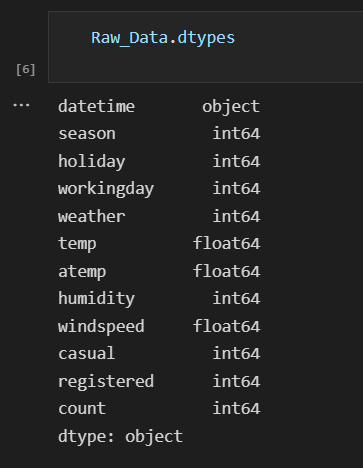
\includegraphics[width=0.2\textwidth]{./figures/DataType.png}
        	\caption{\DIFaddFL{Data Description}}
        	\label{fig:diagram}
        \end{figure}
  \end{itemize}

  \item \DIFadd{Data Outliers Detection }[\DIFadd{\ref{fig:outliers}}]
  \begin{itemize}
    \item \DIFadd{As can been seen in the boxplot }[\DIFadd{\ref{fig:outliers}}]\DIFadd{, there are a number of outliers (e.g., over 800 counts per hour) that can be observed. Therefore, it is necessary to apply a certain rule to remove them, based on the current research standard, the outlier boundaries is ±3 standard deviations from the mean.
         }\begin{figure}[!ht]
        	\centering
        	\setlength{\abovecaptionskip}{0.cm}
        	\setlength{\belowcaptionskip}{-0.cm}
        	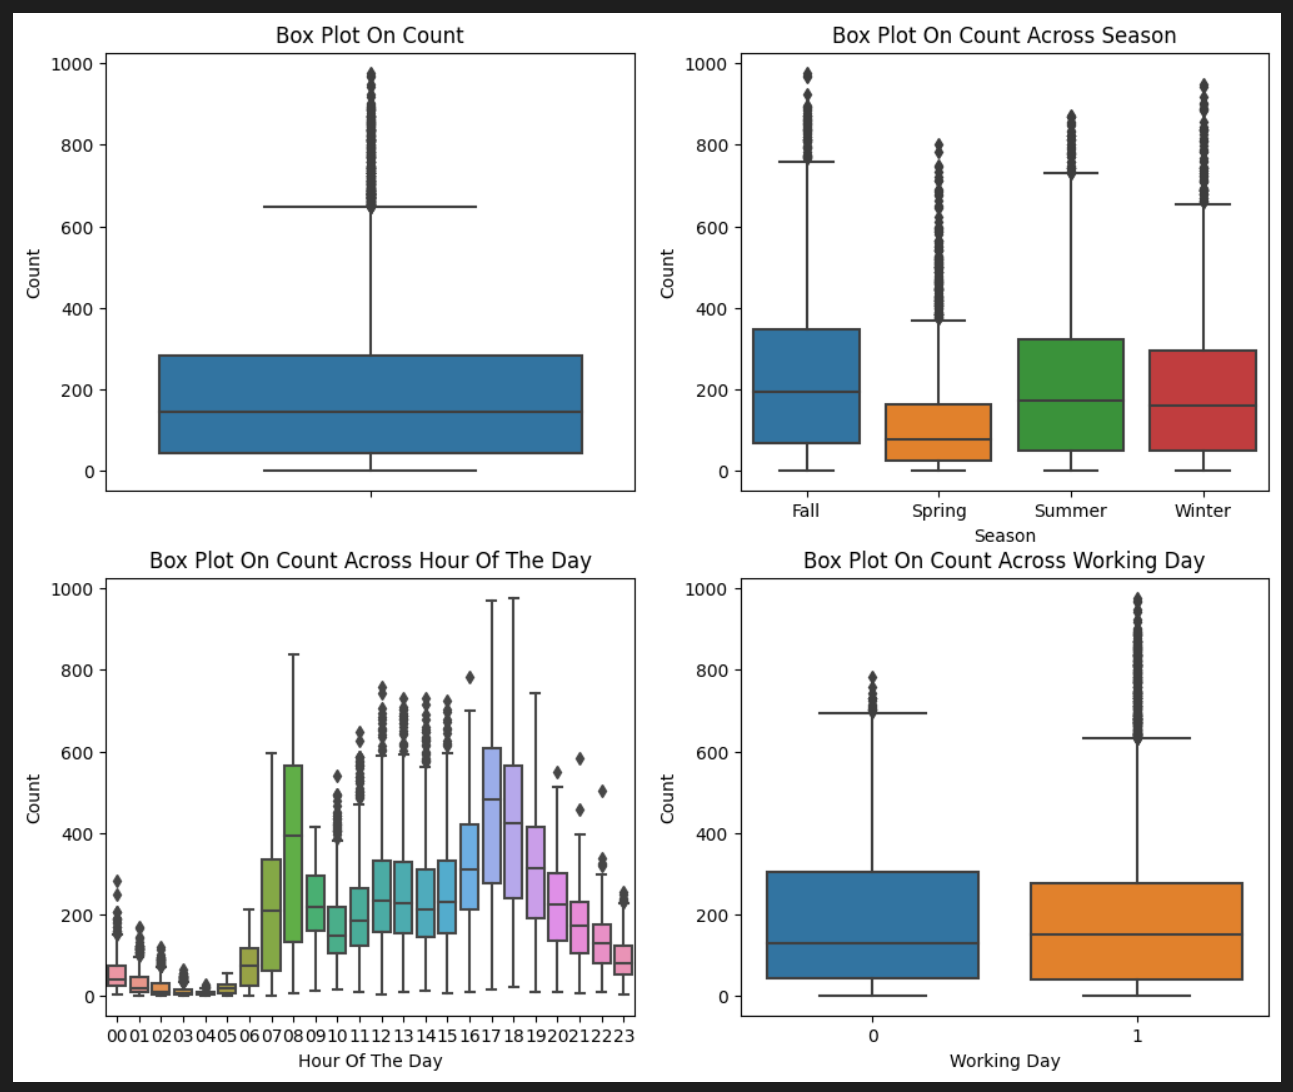
\includegraphics[width=0.3\textwidth]{./figures/DataOutliers.png}
        	\caption{\DIFaddFL{Data Outliers}}
        	\label{fig:outliers}
        \end{figure}
  \end{itemize}

  \item \DIFadd{Correlation Analysis }[\DIFadd{\ref{fig:correlation}}]
   \begin{itemize}
    \item \DIFadd{To further analysis the attributes with numerical data type, as can be seen in }[\DIFadd{\ref{fig:correlation}}]\DIFadd{, the correlation between atemp and temp is too high, which may be considered to drop one of them. Same scenario also happens on the relationship between registered and counts.
     }\begin{figure}[!ht]
    	\centering
    	\setlength{\abovecaptionskip}{0.cm}
    	\setlength{\belowcaptionskip}{-0.cm}
    	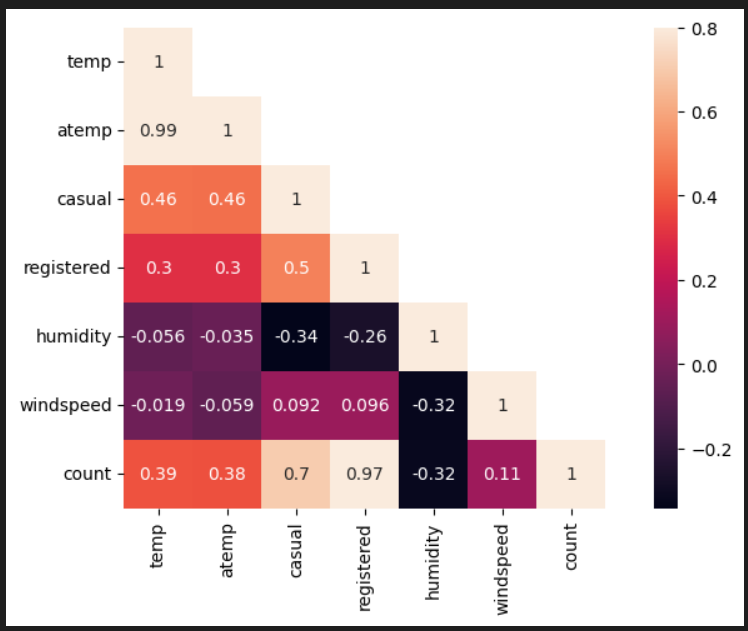
\includegraphics[width=0.3\textwidth]{./figures/Correlation.png}
    	\caption{\DIFaddFL{Correlation}}
    	\label{fig:correlation}
    \end{figure}
  \end{itemize}

  \item \DIFadd{Skewness Distribution}[\DIFadd{\ref{fig:CountDistribution}}][\DIFadd{\ref{fig:windspeed}}]
    \begin{itemize}
        \item \DIFadd{As can be seen in skewness distribution of counts data series can be observed as positive}[\DIFadd{\ref{fig:CountDistribution}}]\DIFadd{, the right tail is much longer than the left tail. It is considered to apply logarithm to reduce the positive skewness.
        }\item \DIFadd{As can be seen in }[\DIFadd{\ref{fig:windspeed}}]\DIFadd{, there are over 1200 records having zero wind speed, which may be a potential problem for prediction accuracy. To avoid the risk, the alternative is to predict these unforeseen zero wind speeds by linear regression
         }\begin{figure}[!ht]
        	\centering
        	\setlength{\abovecaptionskip}{0.cm}
        	\setlength{\belowcaptionskip}{-0.cm}
        	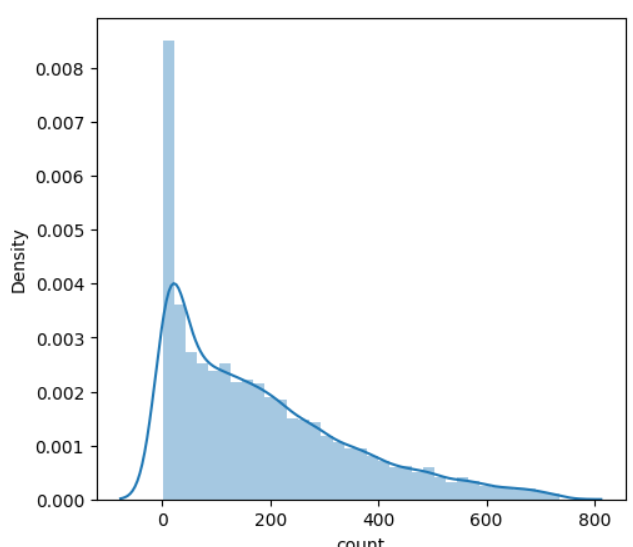
\includegraphics[width=0.3\textwidth]{./figures/CountDistribution.png}
        	\caption{\DIFaddFL{Count Distribution}}
        	\label{fig:CountDistribution}
        \end{figure}
         \begin{figure}[!ht]
        	\centering
        	\setlength{\abovecaptionskip}{0.cm}
        	\setlength{\belowcaptionskip}{-0.cm}
        	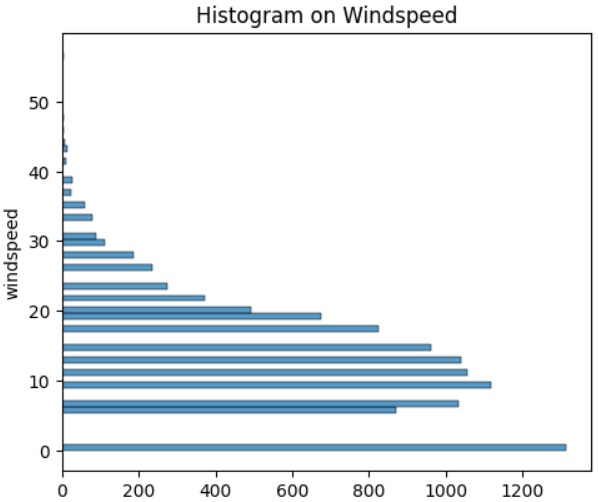
\includegraphics[width=0.3\textwidth]{./figures/windspeed.png}
        	\caption{\DIFaddFL{Windspeed}}
        	\label{fig:windspeed}
        \end{figure}
    \end{itemize}
\end{itemize}

\section{\DIFadd{Method}} \label{sec-method}

\DIFadd{Based on the dataset explored and the problem required to be investigated, the following machine learning algorithms are proposed as potential solutions.
}

\begin{itemize}
    \item \DIFadd{Linear regression - the linear regression fits a linear model with coefficients w = (w1, …, wp) to minimize the residual sum of squares between the observed targets in the dataset, and the targets predicted by the linear approximation. In this case, we can also apply the following two extra methods to increase the accuracy: 1. Use the grid search (GridSearchCV) to exhaustively search over specified parameter values for an estimation; 2. Use the regularization penalty (Ridge) to balance the model prediction by giving an l2-norm regularization.
    }\item \DIFadd{Ensemble Models (averaging or boosting methods) - In averaging methods, the driving principle is to build several estimators independently and then to average their predictions. On average, the combined estimator is usually better than any of the single base estimator because its variance is reduced. By contrast, in boosting methods, base estimators are built sequentially and one tries to reduce the bias of the combined estimator. The motivation is to combine several weak models to produce a powerful ensemble.
}\end{itemize}

\section{\DIFadd{Experiment and Analysis}} \label{sec-experiment}
\DIFadd{In the experiment, the whole process would be elaborated in the following sequence.
}\begin{itemize}
    \item \DIFadd{Feature Engineering: transform datetime attributes into the following four attributes - month, weekday, date, hour; change the meaningless numeric features that we have identified as meaningless into categorical data type, which includes hour, weekday, month, season, weather, holiday, workingday.
    }\item \DIFadd{Outlier Remove and Detection: the outlier boundaries with ±3 standard deviations from the mean should be removed.
    }\item \DIFadd{Skewness Reducing: the positive/negative skewness distribution attribute (i.e., count) should be eliminated by using logarithm, square root, etc.,
}\end{itemize}

\DIFadd{Then, as can be seen in the following four charts, we have visualized the count by month, by the hour of a day with seasons label, by the hour of a day with weekday label, and by the hour of a day with casual/registered label. The obvious trend can be observed that June and July has the highest renting counts, 8 AM and 5 PM reaches the peak of the day for the bike renting in all four seasons and weekdays.
}\begin{figure}[!ht]
	\centering
	\setlength{\abovecaptionskip}{0.cm}
	\setlength{\belowcaptionskip}{-0.cm}
	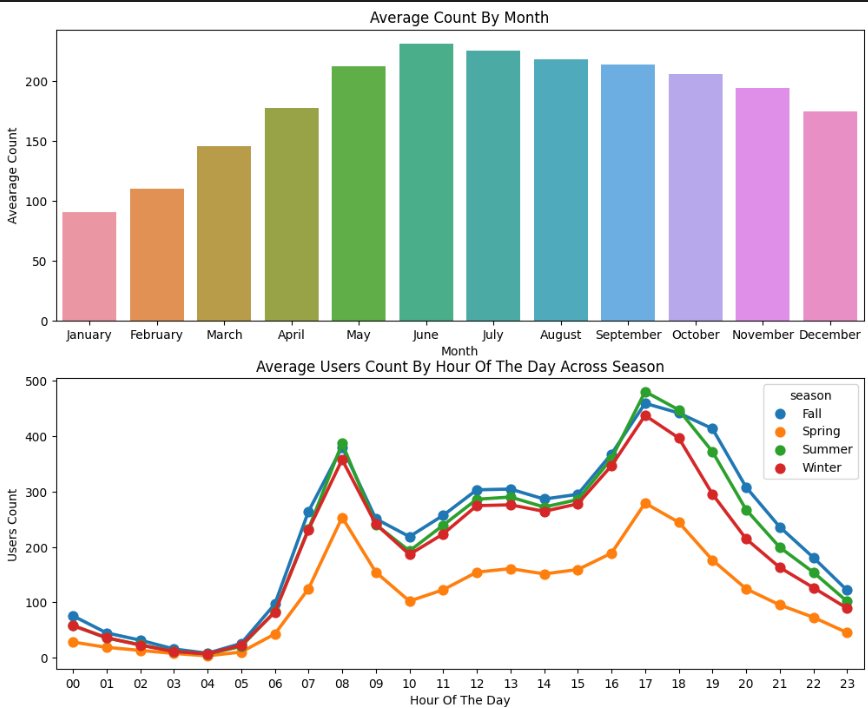
\includegraphics[width=0.5\textwidth]{./figures/Vis-1.png}
	\label{fig:vis-1}
\end{figure}
\begin{figure}[!ht]
	\centering
	\setlength{\abovecaptionskip}{0.cm}
	\setlength{\belowcaptionskip}{-0.cm}
	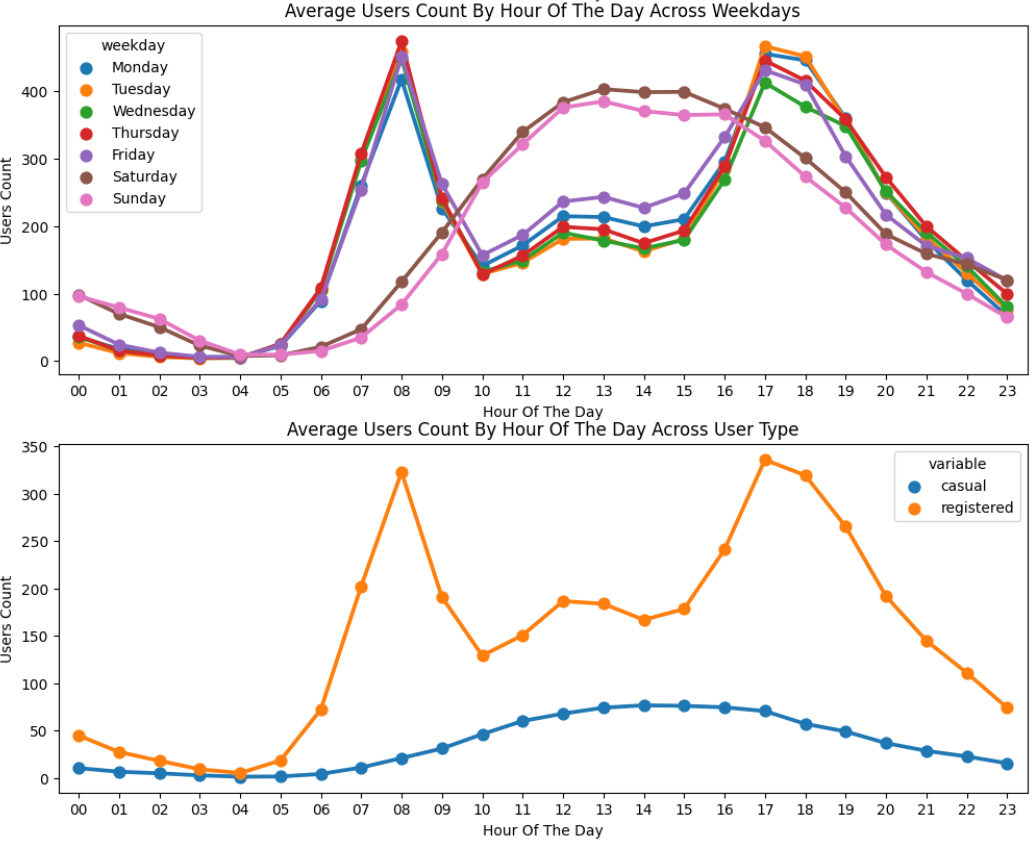
\includegraphics[width=0.5\textwidth]{./figures/Vis-2.png}
	\label{fig:vis-2}
\end{figure}

\DIFadd{Finally, the model would be built and evaluated by using RMSLE.
}\begin{figure}[!ht]
	\centering
	\setlength{\abovecaptionskip}{0.cm}
	\setlength{\belowcaptionskip}{-0.cm}
	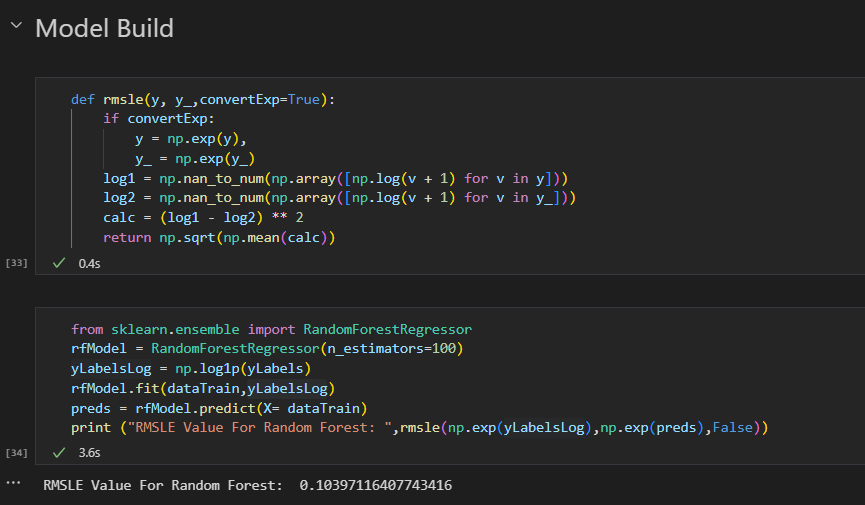
\includegraphics[width=0.7\textwidth]{./figures/model.png}
	\label{fig:model}
\end{figure}

\section{\DIFadd{Conclusions}} \label{sec-conclusions}

\DIFadd{Overall, this report has applied Python to conduct the bike rental forecast during each hour by using the hourly rental data spanning two years. The training set is comprised of the first 19 days of each month, while the test set is from the 20th to the end of the month. Based on the evaluation result provided by RMSLE, the model using random forest has reached the best outcome at a 0.103 RMSLE.
}

 \DIFaddend

% ----------------------------------------------------------------
\bibliography{tuliplab,yourbib}
\bibliographystyle{splncs04}
%=================================================================

%\listoftodos

\end{document}

